\subsection{Boccia}

\begin{enumerate}

\item Essence of Boccia
    \begin{itemize}
    \item Boccia, a precision ball sport, is a captivating display of strategy, accuracy, and finesse.
    \item Athletes with severe physical impairments, often using wheelchairs or assistive devices, compete by propelling or rolling balls towards a target ball, aiming to get their balls closest to the target.
    \item It's a game of tactics and control, requiring players to carefully assess the playing field and execute their throws with precision. 
    \end{itemize}

\item Rules, Equipment, and Competition
    \begin{itemize}
    \item Boccia is played on a flat, rectangular court, with athletes taking turns throwing or rolling their balls towards the target. 
    \item The game can be played individually, in pairs, or in teams, and points are awarded based on the proximity of each ball to the target. 
    \item The sport uses specially designed balls and assistive devices, such as ramps and head pointers, to enable athletes with various impairments to participate fully.
    \end{itemize}

\begin{figure}[htbp] % htbp are float placement options
\centering
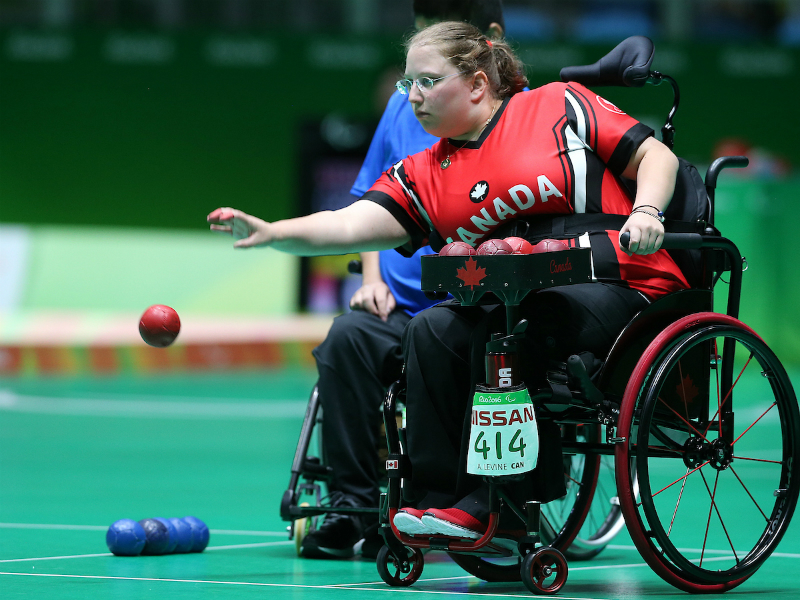
\includegraphics[width=0.8\textwidth]{Images/para_bocce.jpg}
\caption{Para Bocce}
\label{fig:my_image}
\end{figure}

\item Categories and Classifications
    \begin{itemize}
    \item Boccia has a classification system that groups athletes based on the severity of their physical impairments. 
    \item There are four main classifications:
        \begin{itemize}
        \item BC1 for athletes who can throw or kick the ball
        \item BC2 for those who can throw the ball but require assistance with positioning
        \item BC3 for those who cannot throw or kick the ball and use a ramp to propel it
        \item BC4 for athletes with other impairments affecting their coordination and movement
        \end{itemize} 
    \item This system ensures fair competition and allows athletes with diverse abilities to demonstrate their skills and strategies in the sport.
    \end{itemize}

\end{enumerate}